\let\negmedspace\undefined
\let\negthickspace\undefined
\documentclass[journal,12pt,onecolumn]{IEEEtran}
\usepackage{cite}
\usepackage{amsmath,amssymb,amsfonts,amsthm}
\usepackage{algorithmic}
\usepackage{graphicx}
\graphicspath{{./figs/}}
\usepackage{textcomp}
\usepackage{xcolor}
\usepackage{txfonts}
\usepackage{listings}
\usepackage{enumitem}
\usepackage{mathtools}
\usepackage{gensymb}
\usepackage{comment}
\usepackage{caption}
\usepackage[breaklinks=true]{hyperref}
\usepackage{tkz-euclide} 
\usepackage{listings}
\usepackage{gvv}                                        
%\def\inputGnumericTable{}                                 
\usepackage[latin1]{inputenc}     
\usepackage{xparse}
\usepackage{color}                                            
\usepackage{array}                                            
\usepackage{longtable}                                       
\usepackage{calc}                                             
\usepackage{multirow}
\usepackage{multicol}
\usepackage{hhline}                                           
\usepackage{ifthen}                                           
\usepackage{lscape}
\usepackage{tabularx}
\usepackage{array}
\usepackage{float}
%\newtheorem{theorem}{Theorem}[section]
%\newtheorem{theorem}{Theorem}[section]
%\newtheorem{problem}{Problem}
%\newtheorem{proposition}{Proposition}[section]
%\newtheorem{lemma}{Lemma}[section]
%\newtheorem{corollary}[theorem]{Corollary}
%\newtheorem{example}{Example}[section]
%\newtheorem{definition}[problem]{Definition}

\begin{document}

%\textbf{\Large 1.2.1} \\
%\textbf{\large AI25BTECH11001 - Abhisek Mohapatra} \\
\title{4.3.57}
\author{AI25BTECH11001 - ABHISEK MOHAPATRA}
% \maketitle
% \newpage
% \bigskip
%\begin{document}
{\let\newpage\relax\maketitle}
%\renewcommand{\thefigure}{\theenumi}
%\renewcommand{\thetable}{\theenumi}
	 	\textbf{Question}:
		Show that the lines
		\begin{align}
\frac{x-a+d}{\alpha-\delta}=\frac{y-a}{\alpha}=\frac{z-a-d}{\alpha-\delta}
		\end{align}
		\begin{align}
		\frac{x-b+c}{\beta-\delta}=\frac{y-b}{\beta}=\frac{z-b-c}{\beta-\delta}
		\end{align}
are coplanar.
	

	\textbf{Solution:}
		Given:
		\begin{align}
				\vec{L_1} = \vec{A} + \lambda\vec{m_1}
		\end{align}
		\begin{align}
				\vec{L_1} = \myvec{a-d \\a\\a+d} + \lambda
				\myvec{\alpha - \delta\\\alpha\\\alpha + \delta }
		\end{align}And,
		\begin{align}
				\vec{L_2} = \vec{B} + \lambda\vec{m_2}
		\end{align}
		\begin{align}
				\vec{L_2} = \myvec{b-c\\b\\b+c} + \lambda\vec{m_2}
				\myvec{\beta - \delta\\\beta\\\beta + \delta }
		\end{align}
		If the lines lie in a plane, then they satisfy,
		\begin{align}
				nullity\myvec{\vec{m_1}&\vec{m_2}&\vec{B-A}}\geq 1
		\end{align}
		\begin{align}
				nullity\myvec{
						\alpha - \delta & \beta -\delta & a-b+c-d \\
						\alpha & \beta & a-b \\
						\alpha + \delta & \beta +\delta & a-b-c+d
				}\geq 1
		\end{align}
		\begin{align}
				\xrightarrow[]{R_2\leftrightarrow R_3}\myvec{
						\alpha - \delta & \beta -\delta & a-b+c-d \\
						\alpha + \delta & \beta +\delta & a-b-c+d\\
						\alpha & \beta & a-b 
				}
		\end{align}
		\begin{align}
				\xrightarrow[]{R_3\rightarrow R_3-\frac{R_1+R_2}{2}}\myvec{
						\alpha - \delta & \beta -\delta & a-b+c-d \\
						\alpha + \delta & \beta +\delta & a-b-c+d\\
						0 & 0 & 0 
				}
		\end{align}
		\begin{align}
				\xrightarrow[]{R_2\rightarrow R_2-R_1}\myvec{
						\alpha - \delta & \beta -\delta & a-b+c-d \\
						2\delta & 2\delta & -2c+2d\\
						0 & 0 & 0 
				}
		\end{align}
		\begin{align}
				\xrightarrow[]{C_1\rightarrow C_1-C_2}\myvec{
						\alpha - \beta & \beta -\delta & a-b+c-d \\
						0 & 2\delta & -2c+2d\\
						0 & 0 & 0 
				}
		\end{align}
		The matrix is in echelon form and the rank of the matrix is two. And, thus the lines are co-planer.
		

		Graph(using some random values for the variables):
\begin{figure}[h!]
	\centering
	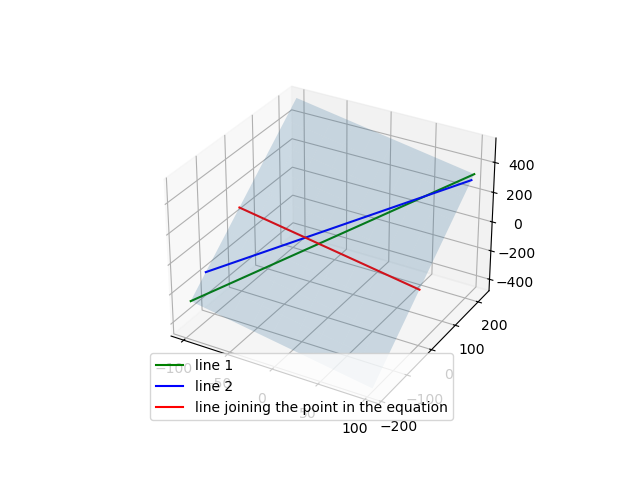
\includegraphics[width=\linewidth]{img.png}
\end{figure}
\end{document}

